\documentclass[main.tex]{subfiles}
\title{Francesca's ciabatta rolls}

\begin{document}

\maketitle% this prints the handout title, author, and date

% \begin{abstract}
% \end{abstract}

\begin{marginfigure}%
  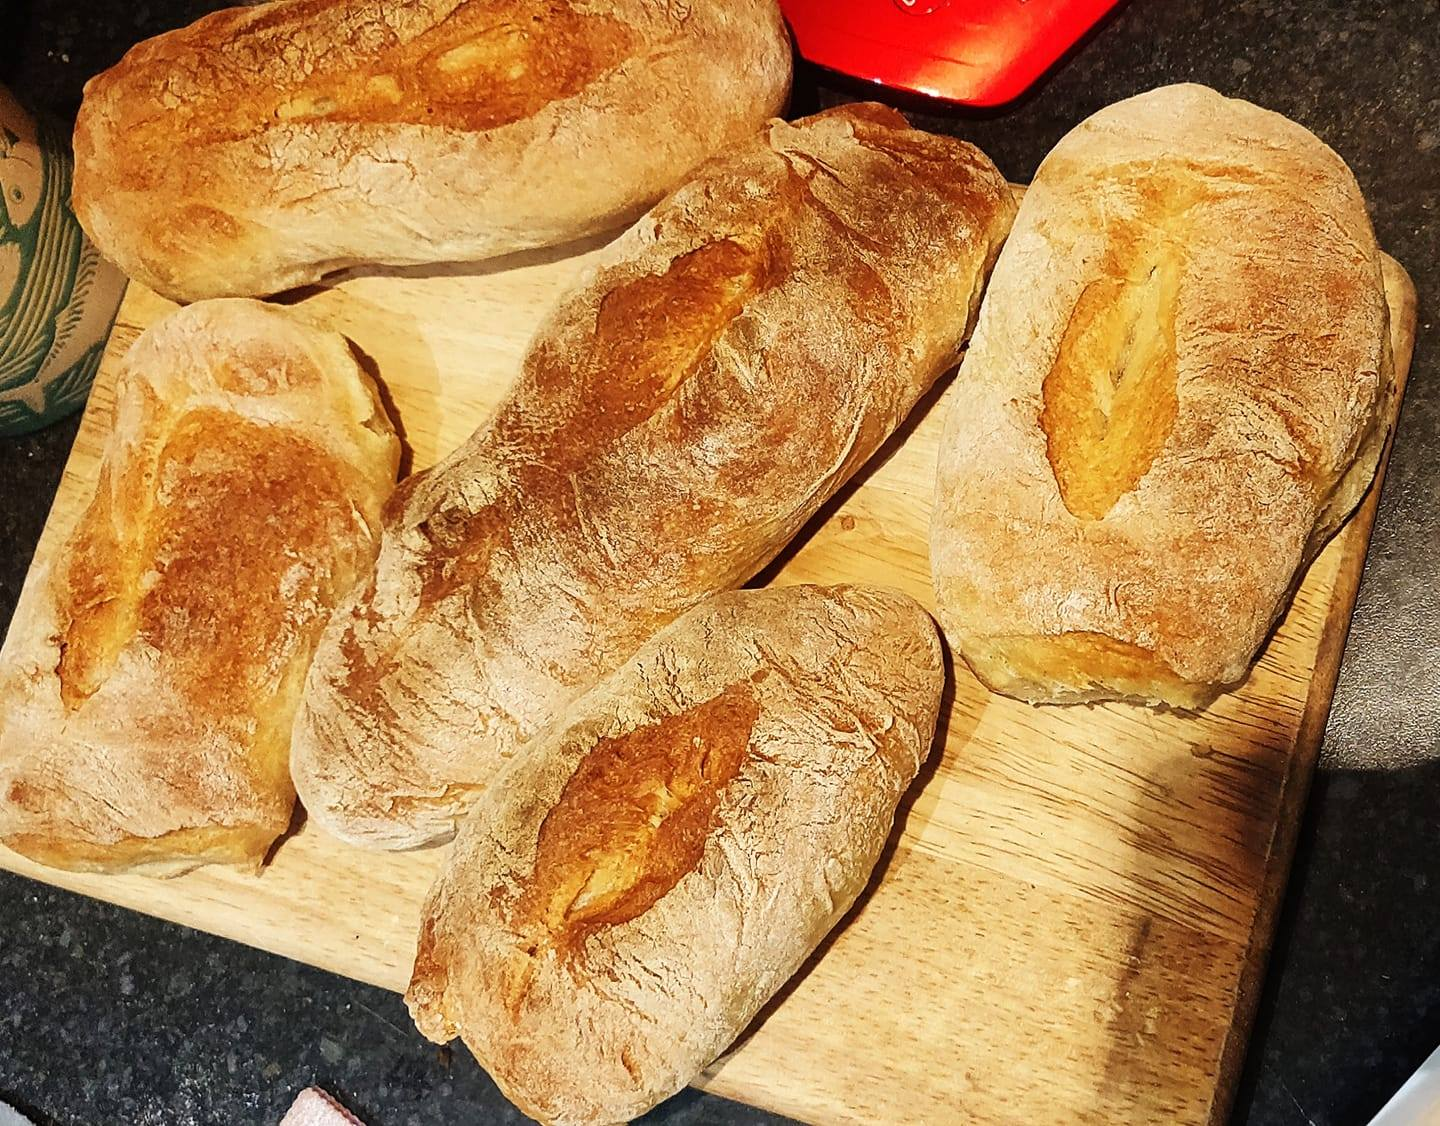
\includegraphics[width=\linewidth]{francesca-ciabatta.jpg}
\end{marginfigure}

\section{Ingredients}

\vspace*{-\baselineskip}
\begin{table}[ht]
	\begin{tabularx}{\textwidth}{>{\hsize=0.333\hsize}X>{\bf\hsize=1\hsize}X}
	\unit[200]{g} & bread flour\\
	\unit[200]{g} & plain flour\\
	\unit[7]{g} & dried yeast\\
	\unit[1]{tsp} & malt powder or honey\\
	\unit[2]{tbsp} & olive oil\\
	\unit[300]{ml} & lukewarm water\\
	\end{tabularx}
\end{table}

\section{Instructions}

NOTE: super wet and sticky dough
\begin{enumerate}
    \item Mix dried ingredients in a big bowl.
    \item Make hole in the middle, add wet ingredients.
    \item Mix together quickly with hands or silicon spatula (recommended).
    \item Cover with clingfilm, let rest for four hours.
    \item Knead for five minutes on a well-floured surface and make into a ball.
    \item Cover with a cloth and let rest an hour.
    \item Divide into four parts.
    \item Pull each into a square or rectangle and fold on itself.
    \item Pat the bread forms into shape, cover with a cloth, let rest forty minutes.
    \item Make a long vertical cut in the top of the rolls. Bake in a \unit[200]{\textdegree C} oven, 20 minutes with a water container at the bottom of the oven, 10 without.
    \item Let cool completely on a wire rack.
\end{enumerate}


% \unit[325]{\textdegree F}

\end{document}
